\documentclass{article} % This command is used to set the type of document you are working on such as an article, book, or presenation
\usepackage{geometry} % This package allows the editing of the page layout
\usepackage{amsmath}  % This package allows the use of a large range of mathematical formula, commands, and symbols
\usepackage{graphicx}  % This package allows the importing of images

\newcommand{\question}[2][]{\begin{flushleft}\textbf{Question #1}: \textit{#2}\end{flushleft}}
\newcommand{\sol}{\textbf{Solution}:} %Use if you want a boldface solution line
\newcommand{\maketitletwo}[2][]{\begin{center}
        \Large{\textbf{Project 1 Report}
        
            Theory of Computer Game} % Name of course here
        \vspace{5pt}
        
        \normalsize{
            Name: Kai-Jie Lin 
            
            Student ID: 110652019
            
            \today}
        \vspace{15pt}
        \end{center}}
\begin{document}
    \maketitletwo[5]  % Optional argument is assignment number
    %Keep a blank space between maketitletwo and \question[1]
    
    \section{Method} 
    The method I use for this game is TD-learning. The feature table is $8 \times 4 \times 6$-tuple network with max tile is 14.
    First, I initialize the value of the table to zero. Then run the game, greedily choose the best policy $\pi$ which is $ \pi (S_{t}) = argmax_{a}(V(S_{t}^{a})) $. 
    $V(S_{t}^{a})$ is the value of taking action $a$ under state $S_{t}$.
    I stored every state of each game in the episode which is a linear data structure. When the game is end, update the value table:  
    $ V(s'_{t}) \leftarrow V(s'_{t}) + \alpha(r_{t+1} + V(s'_{t+1})-V(s'_{t})) $ follow the reversed episode.
    
    \section{Network Design}
    $4\times 6 $-tuple: \\
    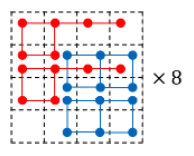
\includegraphics[scale=0.5]{{./tuple.png}} \\
    This is the structure of $4\times 6$-tuple. There are eight different direction, so the total feature number is $8 \times 4$.
    I use isomophic pattern to reduce the weight size. The max tile stored in the feature is 16 (3072).
    \section{Experiment}
    Average score for first one million epoch: \\
    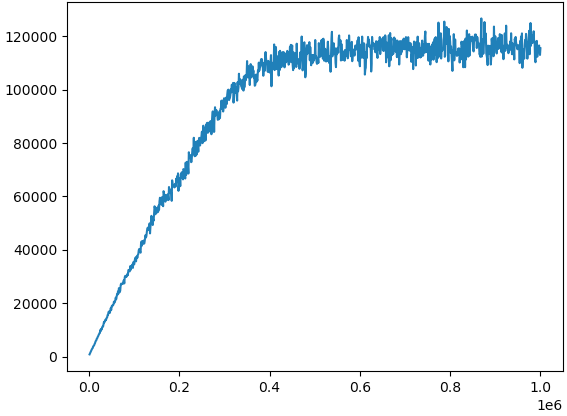
\includegraphics[scale=0.4]{{./training.png}} \\
    I plot the train log for the first one million epoch on the graph using python. I start training with learning rate equals to 0.003125.
    And I got near average score 120000. Then I tuned the learning rate to 0.001 and train for another four million epoch and gradually decrease 
    the learning to 0.0005 and finally 0.00005. I have trained for ten million epoch and the averge score have reached to nearly 2000000. \\
    Sorry for that I did not present the plot of last nine million epoch.
    Because I have forgotten to record the train log during the training process, so the training averge score is discontinuous. 
    I think this will cause some difficulty to analyze the performance, so I did not present it.\\
    Here is the result: \\
    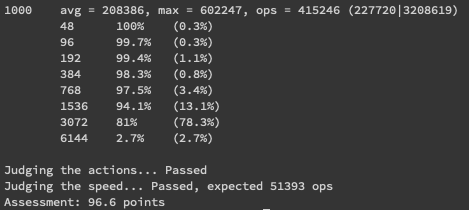
\includegraphics[scale=0.5]{{./result.png}} \\
\end{document}